\documentclass{jarticle}

\usepackage[dvipdfmx]{graphicx}
\usepackage{float}
\usepackage{url}


\title{振り子の運動}
\author{2511198 肥田幸久 \\ 共同実験者 \\ 森嶋和志}
\date{2025年5月29日作成}

\begin{document}
\maketitle



\section{実験の目的}

本実験では、棒振り子の角度のデータから、角度の時間変化の様子、振子の周期
や摩擦の大きさ等を求め、運動を解析する。



\section{実験の原理}

図\ref{fg:rod-pendulum}のような, 金属棒の端点を支点とした棒振り子を考える.

\begin{figure}[H]
  \begin{center}
    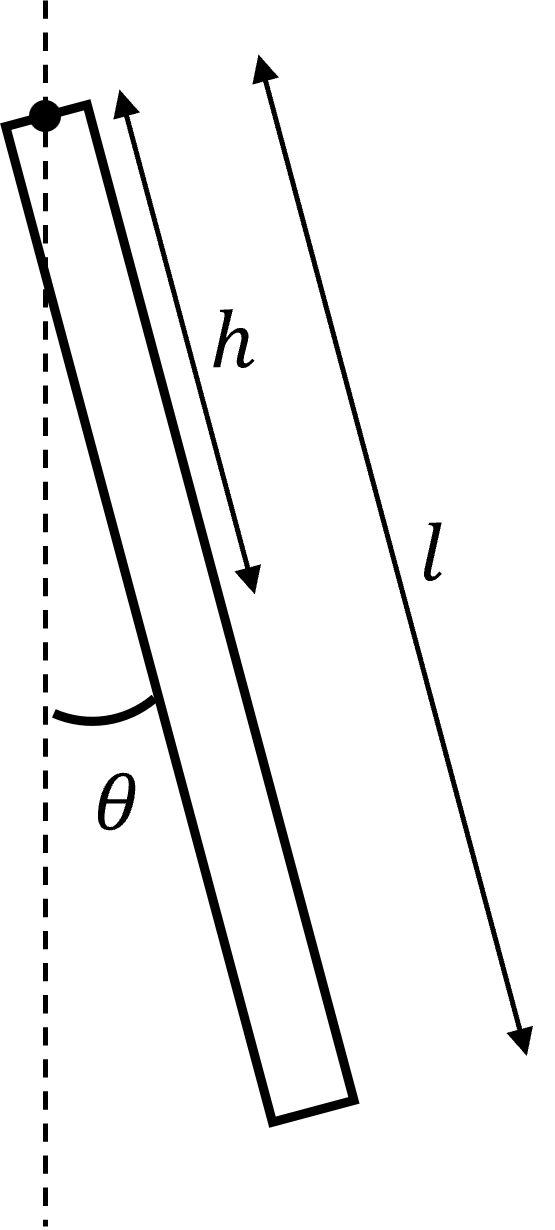
\includegraphics[width=25mm]{rod_pendulum_picture.png}
    \caption{某振り子の運動}
    \label{fg:rod-pendulum}
  \end{center}
\end{figure}

この棒振り子の長さを$l$, 重さを$m$, 振れ角を$\theta(t)$, 支点から棒の重心$(G)$までの長さを$h=l/2$とすると, 運動方程式は次式で表される.
\begin{equation}
  I\frac{d^2\theta}{dt^2}=-mghsin\theta
  \label{eq:EOM-1}
\end{equation}
ここで, $I$は棒の慣性モーメントであり, 棒の端点を回転軸とする際の$I$は,
\begin{equation}
  I=\frac{ml^2}{3}
  \label{eq:MOI}
\end{equation}
で表され, 式(\ref{eq:EOM-1})に代入すると,
\begin{equation}
  \frac{ml^2}{3}\frac{d^2\theta}{dt^2}=-mghsin\theta
  \label{eq:EOM-1.1}
\end{equation}
となる.
また, 摩擦も考慮し粘性摩擦係数を$b$とすると, 運動方程式は,
\begin{equation}
  \frac{ml^2}{3}\frac{d^2\theta}{dt^2}=-mghsin\theta-b\frac{d\theta}{dt}
  \label{eq:EOM-2}
\end{equation}
となり, 整理すると,
\begin{equation}
  \frac{d^2\theta}{dt^2}+\frac{3b}{ml^2}\frac{d\theta}{dt}+\frac{3g}{2l}sin\theta=0
  \label{eq:EOM-2.1}
\end{equation}
と表される.



% \section{実験の原理}

% 振子の振れ幅を$\theta(t)$, 棒の長さを$L$, 棒の重さを$m$, 粘性摩擦係数を$b$とする
% と, 運動方程式は次式になる.

% \begin{equation}
%   \frac{3}{1}mL^2\frac{d^2\theta}{dt^2}+b\frac{d\theta}{dt}+mg\frac{L}{2}sin\theta=0
% \end{equation}

% 整理すると

% \begin{equation}
%   \frac{d^2\theta}{dt^2}+\frac{3b}{mL^2}\frac{d\theta}{dt}+\frac{3g}{2L}sin\theta=0
% \end{equation}

% ここで

% \begin{itemize}
%   \item $\alpha=\frac{3b}{mL^2}$:減衰係数
%   \item $\omega_0=\sqrt{\frac{3g}{2L}}$:非減衰時の自然振動数(大振幅でもおおよその指標になる)
% \end{itemize}



\section{実験方法}

金属棒の端を角度検出センサに取り付け, 棒が振動した際の時間とともに変化する角度に対応したデータ(電圧値)をマイコンで読み取る.
マイコン内に保存されたデータをパソコンに保存し測定データとする.

電圧はセンサの抵抗値が$0\Omega$のとき$0V$, $10k\Omega$のとき電源電圧である$3V$となり, それ
ぞれ角度が$0°$と$360°$に対応している. この電圧値は$10$bit AD変換後の値として記
録されるため, マイコンに記録された角度データの値を$s$とすれば,

\begin{equation}
  \theta=360°\times\frac{s}{2^{10}-1}
\end{equation}

により角度を求めることができる.



\section{実験結果}



\section{考察}


\end{document}

